%\setchapterimage{fig_00}
\chapter*{Colle \arabic{cptColle} \\
 Performances -- \ifprof Corrigé \else Sujet \fi}

\addcontentsline{toc}{section}{Colle \arabic{cptColle} : Performances -- \ifprof Corrigé \else Sujet \fi}

\iflivret \stepcounter{cptColle} \else
\ifprof  \stepcounter{cptColle} \else \fi
\fi
\setcounter{question}{0}

\marginnote{Equipe PT La Martinière Monplaisir.}

%\marginnote{\UPSTIcompetence[2]{B2-04}}
%\begin{marginfigure}
%\centering
%\includegraphics[width=.9\linewidth]{fig_001}
%\end{marginfigure}






On considère la fonction de transfert en boucle ouverte d’un système : $G(p)=\dfrac{8}{p^2+5p+6}$.

\question{Tracer les diagrammes de bode de $G(p)$.}
\ifprof
\begin{corrige}
\end{corrige}
\else
\fi

\question{Tracer la marge de gain et la marge de phase.}
\ifprof
\begin{corrige}
\end{corrige}
\else
\fi

On place ce système dans une boucle de régulation en le précédant d’un correcteur proportionnel $C(p)=K$. La boucle de retour est assurée par un système de fonction de transfert $B(p)=3$.

\question{Tracer le schéma-blocs.}
\ifprof
\begin{corrige}
\end{corrige}
\else
\fi

\question{Calculer la valeur de $K$ de manière à obtenir une marge de phase supérieure ou égale à 45\degres.}
\ifprof
\begin{corrige}
\end{corrige}
\else
\fi

\question{Calculer la valeur de l’écart statique en réponse à un échelon puis en réponse à une rampe.}
\ifprof
\begin{corrige}
\end{corrige}
\else
\fi

On change le correcteur proportionnel, par un correcteur intégral de fonction de transfert $C(p)=Ki/p$.
\question{Calculer la nouvelle valeur de l’écart statique en réponse à un échelon puis en réponse à une rampe.}
\ifprof
\begin{corrige}
\end{corrige}
\else
\fi



\ifprof


\begin{center}
	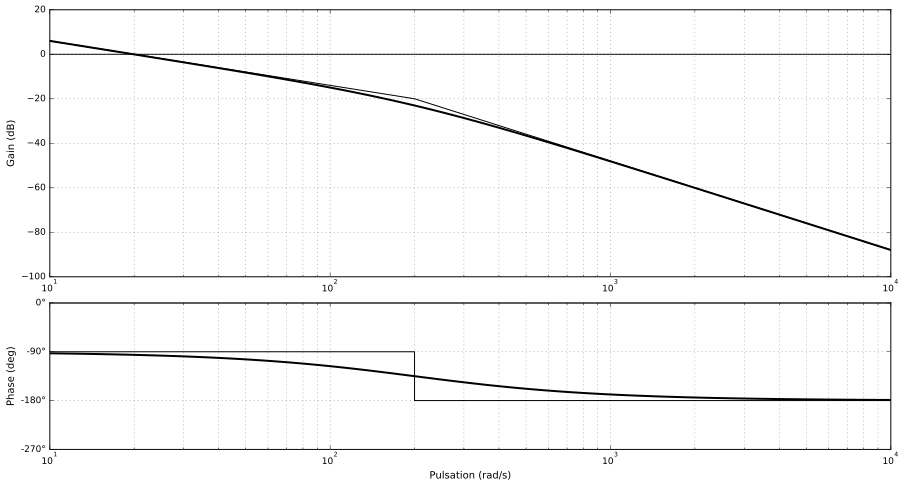
\includegraphics[width=.8\linewidth]{cor_01}
	
	$\varepsilon = 0,123$
	
	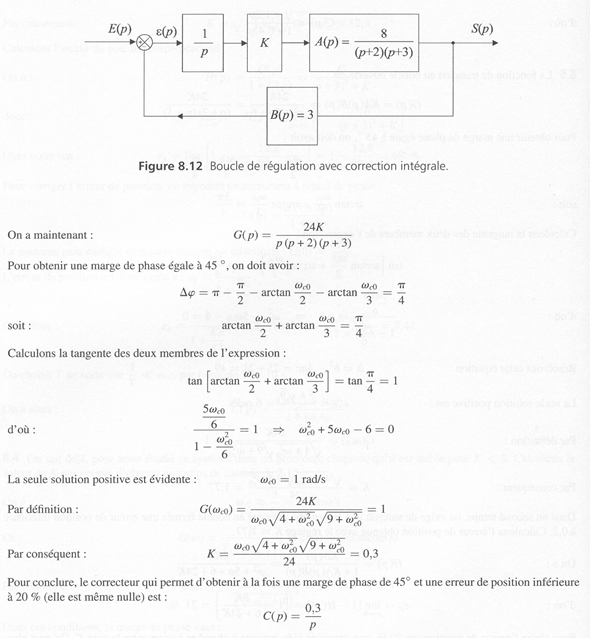
\includegraphics[width=.8\linewidth]{cor_02}
	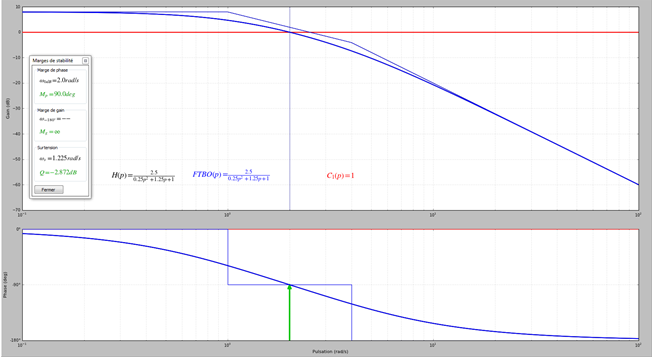
\includegraphics[width=.8\linewidth]{cor_03}
	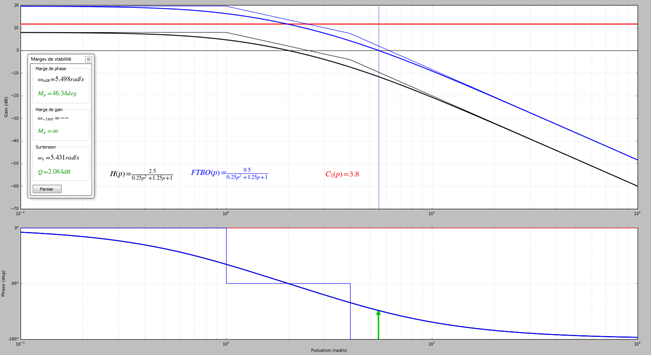
\includegraphics[width=.8\linewidth]{cor_04}
\end{center}

\end{document}


\begin{center}
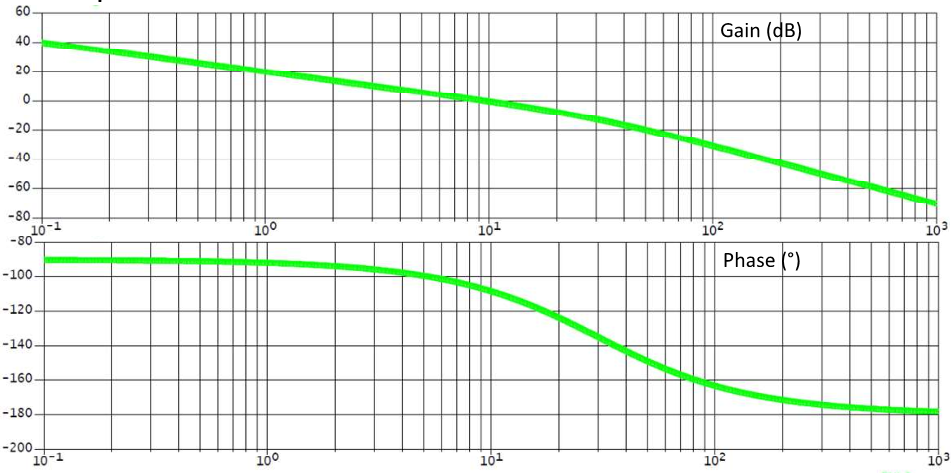
\includegraphics[width=\linewidth]{fig_06}
%\textit{}
\end{center}
\begin{center}
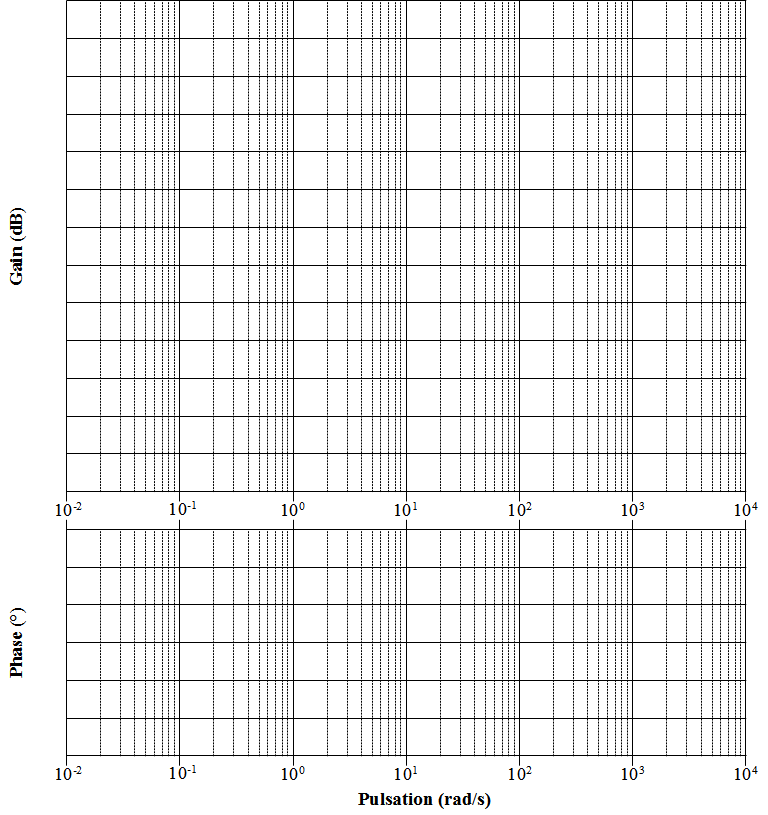
\includegraphics[width=\linewidth]{img_04}
%\textit{}
\end{center}
\else
\fi
